% \documentclass[a4paper, 11pt, titlepage, twoside, openany]{book}
\documentclass[a4paper, 11pt, titlepage, oneside]{book}
\usepackage{plain}
\usepackage{setspace}

\usepackage{threeparttable}
\usepackage{multirow}
\usepackage{booktabs}

\usepackage{float}
\usepackage{makecell}
\usepackage[table]{xcolor}
\usepackage{listings}
\renewcommand{\lstlistingname}{Codice}
% Layout
\usepackage[
  paperheight=29.7cm,
  paperwidth=21cm,
  outer=1.5cm,
  inner=2.5cm,
  top=2cm,
  bottom=2cm
]{geometry}
% Chapter
\usepackage{titlesec}
\singlespacing
\setcounter{secnumdepth}{3}
\setcounter{tocdepth}{3}
% Letter
\usepackage[utf8]{inputenc}
% Language
\usepackage[italian]{babel}
% PDF/A
\usepackage[a-1b]{pdfx}
% Image
\usepackage{graphicx}
\usepackage{wrapfig}
\usepackage{stackengine}
\usepackage{etoolbox}
\BeforeBeginEnvironment{wrapfigure}{\setlength{\intextsep}{0pt}}
% Hyperlink
\usepackage{xurl}
\usepackage[pdfa]{hyperref}
\hypersetup{breaklinks=true}
% Capitalize autoref names
\addto\extrasitalian{%
\renewcommand{\sectionautorefname}{Sezione}%
\renewcommand{\subsectionautorefname}{Sottosezione}%
\renewcommand{\subsubsectionautorefname}{Sottosottosezione}%
}
% List
\usepackage{enumitem}

\lstset{ basicstyle=\ttfamily\small, breaklines=true, backgroundcolor=
\color{gray!10}
, frame=single, rulecolor=
\color{gray}
, captionpos=b, columns=fullflexible, }

\lstset{ language=C, basicstyle=\footnotesize\ttfamily, % <== più piccolo di \small
keywordstyle=
\color{blue}
, commentstyle=
\color{green!60!black}
, stringstyle=
\color{red}
, numberstyle=\tiny
\color{gray}
, numbers=left, frame=single, breaklines=true, breakatwhitespace=false,
showstringspaces=false, captionpos=b % caption sotto il codice
}

\lstdefinestyle{bash}{ language=bash, basicstyle=\footnotesize\ttfamily,
keywordstyle=
\color{blue}
\bfseries, commentstyle=
\color{green!60!black}
\itshape, stringstyle=
\color{red}
, numberstyle=\tiny
\color{gray}
, numbers=left, frame=single, breaklines=true, breakatwhitespace=false, showstringspaces=false,
captionpos=b, morekeywords={sudo, chmod, chown, grep, awk, sed, find, xargs, tar, gzip, curl, wget},
morecomment=[l]{\#}, morestring=[b]", morestring=[b]' }

\lstdefinestyle{changes_in_c}{ language=C, moredelim=**[is][
\color{green!40!black}
]{@}{@} }
% Document
\begin{document}
  % Cover
  \pagenumbering{gobble}
  \pagestyle{plain}
\thispagestyle{empty}

\begin{center}
  \begin{figure}[h!]
    \centering
    
\includegraphics[width=.6\textwidth]{images/logo.pdf}
  \end{figure}

  \vspace{2 cm}
  \LARGE{Dipartimento di Ingegneria e Scienza dell'Informazione\\}

  \vspace{1 cm}
  \Large{Laurea Triennale in\\ Informatica}

  \vspace{2 cm}
  \Large\textsc{Elaborato Finale\\}
  \vspace{1 cm}
  \Huge\textsc{Guida Pratica alla \\Memory-Safety\\}
  \vspace{0.5 em}
  \Large{\textit{}} % Placeholder for correct spacing in "tabular*"

  \vspace{2 cm}
  \begin{tabular*}{\textwidth}{c @{\extracolsep{\fill}} c}
    \Large{Supervisore}             & \Large{Studente}     \\
    \Large{Prof. Silvio Ranise}     & \Large{Isaia Tonini} \\
    \Large{}                        & \Large{234726}       \\
    \Large{Co-Supervisori}          & \Large{}             \\
    \Large{Dott. Pietro De Matteis} & \Large{}             \\
    \Large{Dott. Stefano Berlato}   & \Large{}             \\
  \end{tabular*}

  \vspace{2 cm}
  \Large{Anno accademico 2024/2025}
\end{center}
  \clearpage

  % Acknowledgements
  \thispagestyle{empty}

\begin{center}
  {\bf \Huge Ringraziamenti}
\end{center}

\vspace{4cm}
\emph{Thanks to ...}
  \clearpage
  \pagestyle{plain}

  % Table of Contents
  \frontmatter
  \pagenumbering{Roman}
  \tableofcontents
  \clearpage
  \begingroup
  \pagestyle{empty}
  \cleardoublepage
  \endgroup

  % Start page numbering
  \mainmatter

  % Group to define space between chapters
  \begingroup
  % Override format of title chapter
  \titleformat{\chapter} {\normalfont\Huge\bfseries}{\thechapter}{1em}{} \titlespacing*{\chapter}{0pt}{0.59in}{0.02in}
  \titlespacing*{\section}{0pt}{0.20in}{0.02in} \titlespacing*{\subsection}{0pt}{0.10in}{0.02in}
  \titlespacing*{\subsubsection}{0pt}{0.05in}{0.02in}

  % Abstract
  \chapter*{Sommario}
\label{cha:sommario}
\addcontentsline{toc}{chapter}{Sommario}

La gestione sicura della memoria rappresenta un pilastro fondamentale nella
programmazione moderna e nella cybersecurity, essenziale per prevenire vulnerabilità
ed errori che possono compromettere la stabilità e la sicurezza dei sistemi informatici.
Statistiche recenti mostrano che la maggior parte delle debolezze nelle grandi
codebase è riconducibile a problematiche di \textit{memory safety}, rendendo
questo tema una priorità per la sicurezza del software.

\vspace{0.5em}
\noindent
Questo elaborato si propone di offrire una guida pratica per rafforzare la
sicurezza della memoria lungo l'intero ciclo di vita del software (SDLC). Dopo un'introduzione
al concetto di memory safety, sia dal punto di vista formale che pratico, viene presentata
una panoramica delle principali classi di vulnerabilità (come buffer overflow, use-after-free,
null pointer dereference, etc.) e dei casi reali più rilevanti ad esse associati.
La tesi prosegue con un'analisi approfondita delle tecniche di mitigazione
applicabili nelle diverse fasi dello sviluppo, evidenziandone vantaggi, limiti e
contesti d'uso.

\vspace{0.5em}
\noindent
A supporto degli aspetti teorici, viene presentato un caso studio basato su un'applicazione
C intenzionalmente vulnerabile, analizzata tramite strumenti di analisi statica
e dinamica. L'analisi è proseguita concentrandosi su una vulnerabilità specifica,
per la quale sono state messe a confronto due tecniche di mitigazione: l'adozione
di best practice e l'impiego di librerie esterne specializzate.

\vspace{0.5em}
\noindent
Il contributo principale di questo lavoro consiste nella sistematizzazione delle
tecniche di mitigazione secondo il SDLC e nella dimostrazione pratica della loro
efficacia. L'elaborato si rivolge a studenti e sviluppatori interessati a
ridurre le superfici di attacco e il rischio di incidenti causati da una
gestione non sicura della memoria, fornendo indicazioni operative e strumenti replicabili.

  % Chapters

  \chapter{Introduzione}
\label{cha:introduction}

\section*{Motivazioni e obiettivi}
\label{sec:motivation} La sicurezza della memoria (in inglese, \textit{memory
safety}) è un principio cardine nella programmazione moderna e nella sicurezza
informatica. Essa comprende un insieme di pratiche e tecniche volte a garantire una
gestione sicura della memoria nelle applicazioni, prevenendo errori e
vulnerabilità che potrebbero compromettere l'integrità e la sicurezza del
sistema. La memory safety viene spesso definita come l'assenza di specifiche categorie
di vulnerabilità, quali buffer overflow, use-after-free, null pointer
dereference, etc.. Tuttavia, esistono anche definizioni formali che ne
caratterizzano rigorosamente le proprietà matematiche, che però sono meno diffuse.

Stime di Microsoft\cite{microsoft_proactive_approach} indicano che circa il 70\%
delle vulnerabilità nei loro prodotti deriva da problemi di memory safety.
Analisi di Google\cite{google_memory_safety} riportano percentuali simili per software
come iOS e macOS. Questi dati sottolineano l'importanza di adottare strategie
efficaci per prevenire errori di gestione della memoria prima della messa in
produzione.

Un'ulteriore conferma dell'importanza della memory safety si ricava dalla
classifica \textit{CWE Top 25 Most Dangerous Software Weaknesses}\cite{cwe_top25_2024}
stilata dalla MITRE Corporation\footnote{Sito: https://www.mitre.org/} per il 2024.
Numerose posizioni sono occupate da debolezze legate alla memory safety:
\begin{itemize}
  \item \textbf{CWE-787} Out-of-bounds Write (2° posto): scrittura di dati oltre
    i limiti di un buffer, un array o una struttura dati.

  \item \textbf{CWE-125} Out-of-bounds Read (6° posto): lettura di dati al di fuori
    dei limiti di un buffer, un array o una struttura dati.

  \item \textbf{CWE-416} Use After Free (8° posto): accesso a blocchi di memoria
    deallocati e contrassegnati come liberi, potenzialmente già riutilizzati e
    contenenti dati diversi da quelli precedenti.

  \item \textbf{CWE-119} Improper Restriction of Operations within the Bounds of
    a Memory Buffer (20° posto): mancato controllo dei limiti di un buffer durante
    operazioni di lettura o scrittura (può portare alle CWE-787 e CWE-125).

  \item \textbf{CWE-476} NULL Pointer Dereference (21° posto): dereferenziazione
    di un puntatore nullo.

  \item \textbf{CWE-190} Integer Overflow or Wraparound (23° posto): superamento
    dei limiti di rappresentazione di un intero; non è una vulnerabilità
    direttamente legata alla memoria, ma può causare errori di allocazione o accesso
    a memoria se non gestita correttamente.
\end{itemize}
La persistenza e la gravità delle vulnerabilità legate alla gestione della
memoria ne fanno una delle principali cause sia di exploit attivi che di
incidenti su scala globale.

\bigskip
\noindent
Due casi emblematici, accaduti a distanza di anni ma accomunati dalla natura della
vulnerabilità, aiutano a comprendere l'importanza critica della memory safety: uno
riguarda una debolezza strutturale del linguaggio e dell'ecosistema in cui è stato
scritto il software; l'altro evidenzia come anche in ambienti moderni, apparentemente
più sicuri, l'errore umano possa portare a conseguenze disastrose. In entrambi gli
episodi, la gestione inadeguata della memoria ha costituito il fattore
scatenante, ma l'impatto devastante è stato amplificato dai privilegi di esecuzione
elevati dei software coinvolti: entrambi operano infatti a livello di kernel, dove
gli errori di memoria possono compromettere l'intero sistema operativo.

\paragraph{WannaCry (maggio 2017)}

L'attacco ransomware\footnote{Tipo di malware che cripta i file del sistema
vittima e richiede un riscatto per fornire la chiave di decrittazione} WannaCry
sfruttò una vulnerabilità di \textit{buffer overflow} nel protocollo SMBv1\footnote{Protocollo
di rete utilizzato per la condivisione di file, stampanti e altre risorse tra dispositivi
in una rete} di Windows, nota come EternalBlue (CVE-2017-0144), che corrisponde
alla debolezza CWE-787 (Out-of-bounds Write)\footnote{Dettagli del codice: https://www.scademy.com/the-legacy-code-behind-wannacry-the-skeleton-in-the-closet/,
ultimo accesso: 17 giugno 2025}. Microsoft aveva rilasciato una patch di
sicurezza per questa vulnerabilità nel marzo 2017, ma molti sistemi rimasero non
aggiornati, permettendo al malware di propagarsi rapidamente. Si trattava di una
tipica debolezza legata alla gestione della memoria, comune in software scritto
in C/C++, in cui il controllo sui limiti dei buffer è lasciato completamente al programmatore.

Il malware infettò oltre 300.000 computer in oltre 150 Paesi, criptando i dati e
richiedendo un riscatto in Bitcoin. Tra le vittime più colpite vi fu il Servizio
Sanitario Nazionale del Regno Unito (NHS), che dovette cancellare migliaia di
appuntamenti e deviare ambulanze, con un impatto stimato di circa 92 milioni di sterline.
I danni economici globali furono stimati fino a 4 miliardi di dollari.\cite{wannacry_kaspersky}

L'attacco evidenzia come l'utilizzo di linguaggi a gestione manuale della memoria,
come C e C++, possa esporre i sistemi a vulnerabilità critiche quando non vengono
adottate pratiche rigorose di sicurezza e aggiornamento tempestivo.

\paragraph{CrowdStrike Falcon Sensor (luglio 2024)}

Recentemente, un aggiornamento difettoso del software di sicurezza CrowdStrike
Falcon Sensor ha causato malfunzionamenti e blocchi di sistema su vasta scala, colpendo
circa 8,5 milioni di dispositivi aventi installato Windows. L'incidente è stato
causato da un errore di accesso alla memoria (lettura \textit{out-of-bounds}) nel
codice, corrispondente alla debolezza CWE-125 (Out-of-bounds Read), sfuggito ai controlli
e ai test prima del rilascio.\cite{crowdstrike2024incident}

L'incidente ha paralizzato infrastrutture critiche in diversi settori come
compagnie aeree, banche e strutture sanitarie, con danni economici stimati
intorno ai 15 miliardi di dollari.\cite{crowdstrike_bug_wired_cost}

Questo episodio dimostra come anche errori interni nei software, derivanti da
sviste umane nella gestione della memoria, possano generare conseguenze disastrose
a livello internazionale, evidenziando che la memory safety rimane un requisito
critico anche per i sistemi più avanzati e affidabili.

\bigskip
\noindent
I principali contributi di questo elaborato sono:
\begin{itemize}
  \item L'\textbf{analisi critica} delle tecniche di mitigazione secondo le fasi
    del SDLC, fornendo un framework operativo per introdurre la sicurezza \textit{by
    design}.

  \item La \textbf{dimostrazione pratica} dell'efficacia e delle limitazioni
    degli strumenti di analisi attraverso un caso di studio replicabile su un'applicazione
    C vulnerabile.

  \item Il \textbf{confronto} tra approcci di mitigazione (best practice vs.
    librerie specializzate) con valutazione di vantaggi/svantaggi per diversi contesti
    applicativi.
\end{itemize}

\section*{Struttura del lavoro}
\label{sec:structure} La tesi è divisa in quattro capitoli principali. Inizialmente,
viene fornita una panoramica generale del concetto di memory safety e di quali
siano le principali vulnerabilità legate alla memoria (\autoref{cha:background}).

Successivamente, vengono illustrate tecniche di mitigazione per rafforzare la memory
safety, dividendole tra le varie fasi del ciclo di vita del software, dalla progettazione
al mantenimento (\autoref{cha:sdlc}).

Il terzo capitolo è dedicato a un caso di studio pratico, in cui viene
presentata un'applicazione scritta in C con vulnerabilità di memory safety. Viene
illustrato il processo di analisi e correzione delle vulnerabilità, utilizzando
strumenti e tecniche discusse nei capitoli precedenti (\autoref{cha:real_case}).

Infine, il capitolo conclusivo prevede una sintesi dei risultati ottenuti e l'esplorazione
di possibili sviluppi futuri, con l'obiettivo di migliorare ulteriormente la
memory safety nei progetti software (\autoref{cha:conclusioni}).

  \chapter{Background}
\label{cha:background}

In questa sezione vengono fornite le nozioni fondamentali necessarie per
comprendere il tema della memory safety e il suo impatto nello sviluppo software.

Vengono quindi chiariti i principi di base legati alla memory safety, le tipologie
più comuni di vulnerabilità dovute a una gestione scorretta della memoria, e il
modo in cui tali vulnerabilità possano impattare l'integrità di sistemi reali. Questa
analisi fornisce il contesto necessario per comprendere l'importanza delle tecniche
e degli strumenti di mitigazione che sono presentati nei capitoli successivi.

% Definizione di memory safety
\section{Definizione di memory safety}
\label{sec:memory_safety}

Il concetto di memory safety non dispone di una definizione formale univoca,
generalmente riconosciuta da tutta la comunità scientifica. In letteratura si trovano,
per la maggior parte, definizioni di carattere più pratico, che si concentrano
sull'assenza di determinati tipi di bug o comportamenti indesiderati legati alla
gestione della memoria.

Di seguito, vengono presentate sia una definizione formale di memory safety che una
definizione intuitiva derivante da aspetti più pratici, al fine di fornire una
visione completa del concetto e delle sue implicazioni.

\paragraph{Definizione formale}

Una delle definizioni formali di memory safety più accreditate è quella proposta
da A. Azevedo de Amorim et al.~\cite{meaning_memory_safety}, che si basa su una
formalizzazione rigorosa del concetto, attraverso un framework matematico basato
su semantica operazionale e strutture formali per ragionare sulla sicurezza della
memoria in modo verificabile.

Nel modello proposto, un programma è considerato \textbf{memory safe} se,
durante la sua esecuzione, preserva le seguenti proprietà:
\begin{enumerate}
  \item \textbf{Isolamento spaziale e temporale}:
    \begin{itemize}
      \item Le operazioni su una regione di memoria non influenzano dati al di fuori
        del proprio ``footprint'' (porzione accessibile).

        \textit{Per esempio, gli accessi out-of-bound violano questa proprietà,
        poiché le porzioni di memoria fuori dai limiti di un array non fanno
        parte del suo footprint}

      \item I \textit{Frame Theorems}, sviluppati e dimostrati in~\cite{meaning_memory_safety},
        garantiscono che l'estensione dello heap iniziale con blocchi non
        raggiungibili non alteri il comportamento del programma.
    \end{itemize}

  \item \textbf{Non-interferenza}:
    \begin{itemize}
      \item Nel modello ideale proposto, la memoria non raggiungibile non può
        modificare né essere modificata durante l'esecuzione. Ciò assicura sia \textit{integrità}
        (impossibilità di alterare dati isolati), sia \textit{segretezza} (impossibilità
        di dedurne l'esistenza).
    \end{itemize}

  \item \textbf{Contenimento degli errori}:
    \begin{itemize}
      \item Accessi illegali (es. dereferenziazione di puntatori invalidi)
        terminano l'esecuzione in modo prevedibile con un errore esplicito, evitando
        comportamenti indefiniti.
    \end{itemize}
\end{enumerate}

Questo modello consente di dimostrare proprietà come la protezione tra moduli e l'assenza
di comportamenti indefiniti. Conseguentemente, esso fornisce anche un solido framework
matematico per specificare e dimostrare le garanzie di sicurezza implementate da
un sistema (come proprietà del \textit{type system} o del \textit{memory model}).
Tale formalizzazione guida inoltre lo sviluppo di strumenti verificati per l'enforcement
della memory safety, come i monitor hardware/software descritti in~\cite{meaning_memory_safety}.

Tuttavia, questa definizione si basa su ipotesi idealizzate, come memoria illimitata,
assenza di side-channel\footnote{Canale d'informazione non intenzionale che
permette di estrarre dati sensibili attraverso l'osservazione di caratteristiche
fisiche o temporali del sistema (es. consumo energetico, timing delle operazioni,
emissioni elettromagnetiche) piuttosto che attraverso l'accesso diretto ai dati.}
sfruttabili dagli attaccanti e assenza di aritmetica sui puntatori o di cast a interi
(che permettono la manipolazione diretta degli indirizzi), che lo rendono
parzialmente allineato ai linguaggi e agli ambienti reali. Per questo motivo una
definizione più intuitiva e pratica può essere utile per comprendere il concetto
di memory safety in contesti reali.

\paragraph{Definizione pratica}

Dal punto di vista pratico, la memory safety viene comunemente intesa come la
capacità di un programma di evitare vulnerabilità o comportamenti errati legati
alla gestione della memoria.

Una definizione operativa in questo senso è fornita da D. Dhurjati et al.~\cite{memory_safety_without_runtime_checks},
che descrivono un programma memory safe come un'entità software che:
\begin{itemize}
  \item non accede a locazioni di memoria al di fuori dello spazio di indirizzamento
    a esso allocato;

  \item non esegue istruzioni al di fuori del proprio codice compilato e ``linkato''
    (ovvero del codice risultante dal collegamento con le librerie statiche e
    dinamiche)

  \item rispetta restrizioni di tipo sulle operazioni, vincoli sulle conversioni
    di tipo e accessi nei limiti degli array.
\end{itemize}

Sulla base di questi principi, la memory safety può essere vista come la capacità
di garantire che tutte le operazioni di accesso alla memoria (lettura, scrittura,
esecuzione) avvengano in modo controllato e conforme alle intenzioni del programma.
In altre parole, essa protegge il programma da errori come \textit{buffer
overflow}, \textit{dangling pointers} e \textit{use after free}, che possono
causare violazioni di integrità o problemi di sicurezza.

Questa visione, pur derivando da un'analisi formale, si allinea con un'intuizione
più diffusa: un programma è memory safe se è protetto da una serie di bug comuni
e pericolosi relativi agli accessi in memoria. Questa prospettiva è spesso
adottata in contesti divulgativi, dove la memory safety è intesa come l'assenza di
specifiche classi di vulnerabilità anziché come una proprietà rigorosamente formale.

% Memory Safety Continuum %
\paragraph{Memory safety come spettro continuo}

Il divario tra modelli teorici e implementazioni reali suggerisce che la memory safety
non sia una proprietà assoluta o binaria, ma una condizione che può essere
raggiunta in misura variabile in contesti di applicazione reali.

Mentre la definizione formale fornisce garanzie assolute all'interno del proprio
modello matematico, le limitazioni e le idealizzazioni di tale modello rendono difficile
il raggiungimento di una memory safety completa nei sistemi pratici.

Questa idea viene esplicitamente sviluppata dalla \textit{Open Source Security
Foundation} (OpenSSF)~\cite{memory_safety_continuum}, che propone di interpretare
la memory safety come uno spettro continuo. In tale visione, sistemi e linguaggi
possono offrire livelli differenti di protezione, a seconda delle garanzie fornite
e delle mitigazioni adottate.

Questo approccio sottolinea come la memory safety possa essere rafforzata progressivamente,
piuttosto che garantita in modo assoluto.

% Tipi di vulnerabilità
\section{Tipi di vulnerabilità}
\label{sec:vulnerability_types}

Esistono diverse classificazioni per le vulnerabilità legate alla memoria, che
esplorano le debolezze in modo molto specifico relazionandole tra loro, come quella
proposta da MITRE (CWE-1399\cite{cwe_1399}). Tuttavia, per fornire una visione d'insieme
delle vulnerabilità più comuni, questa sezione propone la tassonomia sviluppata da
OpenSSF\cite{memory_safety_continuum_definition}.

La classificazione in questione organizza le vulnerabilità di memory safety in
quattro categorie principali: errori di accesso, variabili non inizializzate, memory
leak e race condition.

\begin{quote}
  \textbf{Nota:} La nomenclatura utilizzata in questa sezione può differire da
  quella impiegata nell'introduzione (come "buffer overflow" e "out-of-bounds
  write"). Queste variazioni riflettono semplicemente modi diversi di denominare
  le stesse vulnerabilità, dipendendo dal livello di specificità desiderato e
  dalle fonti di riferimento adottate. Per coerenza, sono stati mantenuti i
  termini presenti nelle rispettive fonti citate; per una nomenclatura più precisa
  e sistematica si rimanda alla classificazione CWE-1399\cite{cwe_1399}.
\end{quote}

\paragraph{Errori di accesso (Access errors)}
\label{sec:access_errors}

Comprendono tutte le operazioni di lettura o scrittura invalide di un puntatore
che violano i confini o lo stato di validità della memoria:
\begin{itemize}
  \item \textbf{Buffer overflow} (CWE-787): scrittura oltre la capacità di un buffer.

  \item \textbf{Buffer over-read} (CWE-125): lettura oltre i limiti di un buffer.

  \item \textbf{Invalid page fault}: accesso a pagine di memoria non valide.

  \item \textbf{Use after free} (CWE-416): accesso a blocchi di memoria dopo la loro
    deallocazione.
\end{itemize}
Un caso emblematico è la vulnerabilità \textit{Heartbleed}\cite{heartbleed} scoperta
nel 2014 in OpenSSL che, attraverso un buffer over-read, causò una massiccia fuga
di dati da server web. Anche i casi di WannaCry e CrowdStrike (introdotti precedentemente)
sono legati a vulnerabilità di accesso.

\paragraph{Variabili non inizializzate (Uninitialized variables)}
\label{sec:uninitialized}

Riguardano l'uso di variabili che non sono state assegnate con un valore valido:
\begin{itemize}
  \item \textbf{Null pointer dereference} (CWE-476): dereferenziazione di puntatori
    nulli.

  \item \textbf{Wild pointers}: puntatori con valori casuali o invalidi.

  \item \textbf{Uninitialized variables}: uso di variabili prima della loro inizializzazione.
\end{itemize}
Un caso significativo per tali bug è quello del kernel Linux\cite{null_pointer_dereference_linux},
che ha mostrato come una dereferenziazione di puntatore nullo possa permettere escalation
di privilegi e Denial of Service.

\paragraph{Memory leak}
\label{sec:memory_leaks}

Comprendono situazioni in cui l'uso della memoria non è tracciato correttamente o
viene tracciato in modo errato:
\begin{itemize}
  \item \textbf{Stack exhaustion}: esaurimento dello spazio disponibile nello stack.

  \item \textbf{Heap exhaustion}: esaurimento dello spazio disponibile nell'heap.

  \item \textbf{Double free}: doppia liberazione della stessa area di memoria.

  \item \textbf{Invalid free}: tentativo di liberare memoria non allocata.

  \item \textbf{Mismatched free}: uso di funzioni di deallocazione incompatibili.

  \item \textbf{Unwanted aliasing}: riferimenti multipli non intenzionali alla stessa
    area.
\end{itemize}
Per questa categoria, si può fare riferimento al double free presente in WhatsApp
scoperto nel 2019\cite{whatsapp_double_free}, che permetteva l'esecuzione di codice
arbitrario tramite l'invio di una GIF malformata.

\paragraph{Race condition}
\label{sec:race_conditions}

Sebbene le race condition riguardino accessi concorrenti a memoria condivisa e possano
causare comportamenti non deterministici che compromettono la memory safety,
esse spaziano oltre il focus specifico di questa tesi. Vengono pertanto menzionate
per completezza, ma non vengono trattate in dettaglio nei capitoli successivi.

  \chapter{Memory Safety nel SDLC}
\label{cha:sdlc}

Dopo aver introdotto i concetti fondamentali legati alla memory safety e aver
visto l'impatto che una gestione errata della memoria può avere sulla sicurezza,
sull'affidabilità e sulla stabilità del software, questo capitolo si concentra
su come questi principi possano essere concretamente integrati all'interno del
ciclo di vita dello sviluppo del software \textit{(Software Development Life Cycle,
SDLC)}(\autoref{fig:sdlc_img}).

\begin{figure}[htbp]
  \centering
  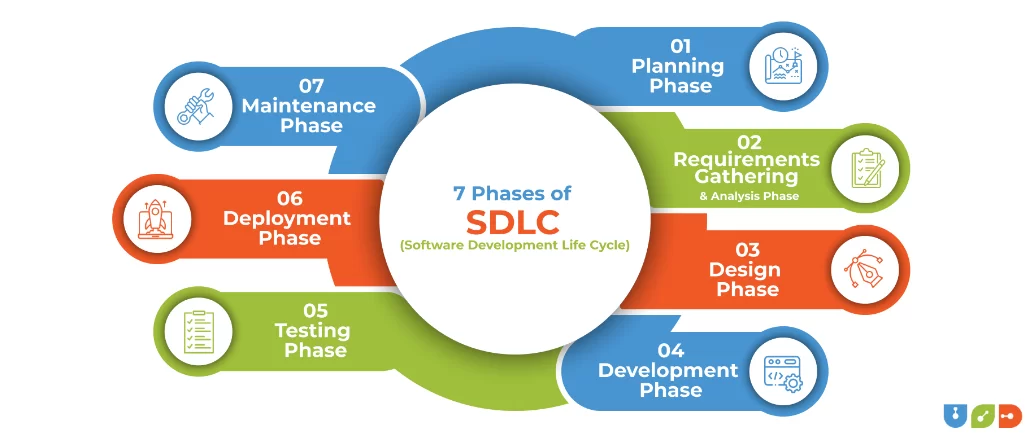
\includegraphics[width=0.7\textwidth]{images/sdlc.png}
  \caption[Schema SDLC]{Schema SDLC\protect\footnotemark}
  \label{fig:sdlc_img}
\end{figure}
\footnotetext{Fonte: \url{https://uniquesoftwaredev.com/the-software-development-life-cycle-sdlc-7-phases-and-models/}}

Diversi studi nella letteratura confermano che la sicurezza del software non può
essere trattata come un'attività relegata alle fasi finali del ciclo di sviluppo.
In particolare, secondo la revisione sistematica di Chin Eian et al.\cite{security_in_sdlc},
una delle principali conclusioni è che l'integrazione degli aspetti di sicurezza
all'interno di tutte le fasi del SDLC è essenziale per ridurre il rischio di
introdurre vulnerabilità gravi e costose da mitigare nelle fasi successive. In linea
con questa visione, il seguente capitolo analizza come i principi di \textit{memory
safety} possano essere incorporati concretamente lungo l'intero ciclo di vita dello
sviluppo software, piuttosto che essere considerati come un'attività isolata o
relegata a una fase finale.

Va sottolineato fin da subito che le tecniche, gli strumenti e i linguaggi eventualmente
citati \textit{non} vanno intesi come universali o necessariamente ottimali per
ogni contesto. L'obiettivo di questo capitolo non è infatti quello di raccomandare
soluzioni specifiche, ma piuttosto fornire un \textit{quadro strutturato di
buone pratiche e approcci} che possono essere adattati in base ai requisiti del progetto,
alle risorse disponibili e al contesto applicativo.

\section{Pianificazione, Analisi dei Requisiti e Design}
\label{sec:planning_requirements_design}

Le fasi preliminari del \textit{Software Development Life Cycle} (SDLC)
comprendono l'analisi dei requisiti, la pianificazione e il design del software.
Sebbene queste attività non prevedano ancora la scrittura effettiva del codice, rivestono
un ruolo cruciale nella definizione delle proprietà di sicurezza dell'intero sistema,
incluse le garanzie di \textit{memory safety}.

Una corretta impostazione in queste fasi consente di identificare precocemente i
rischi legati all'uso della memoria e di predisporre adeguate strategie di mitigazione.
Ad esempio, in un progetto che prevede l'implementazione di algoritmi crittografici,
è fondamentale orientare le scelte tecniche (come linguaggi e librerie) verso
strumenti che riducano al minimo la possibilità di errori di memoria. Una gestione
errata in questo ambito può esporre l'applicazione a vulnerabilità gravi, come
la possibilità di decrittare dati sensibili o di compromettere l'integrità del
sistema.

In particolare, già in fase di progettazione è possibile (e raccomandabile) condurre
un'analisi dei requisiti di sicurezza, esplicitando obiettivi orientati alla
\textit{memory safety}. Analogamente, durante la fase di pianificazione, è utile
prevedere misure difensive trasversali all'intero ciclo di vita, come l'uso di ambienti
\textit{sandbox} durante il deployment per limitare i danni derivanti da
eventuali vulnerabilità di memoria. Questi requisiti e decisioni guideranno poi tutte
le fasi successive dello sviluppo.

\subsection{Scelta del Linguaggio}
\label{sec:linguaggio}

La scelta del linguaggio di programmazione rappresenta una delle decisioni
fondamentali nelle fasi preliminari dello sviluppo software. Essa influenza in modo
diretto la qualità, la sicurezza e la manutenibilità del codice prodotto, ed è particolarmente
rilevante quando si vogliono prevenire vulnerabilità legate alla \textit{memory
safety}.

Sebbene linguaggi come Rust siano stati progettati con l'obiettivo esplicito di
garantire la \textit{memory safety}, non esiste una soluzione unica valida per
tutti i contesti. Ogni linguaggio presenta compromessi progettuali che ne influenzano
l'idoneità in scenari specifici.

Per esempio, C e C++ restano la scelta dominante nello sviluppo di firmware, driver
o sistemi embedded, dove è richiesto un controllo a basso livello dell'hardware
e delle risorse. Al contrario, Java e Kotlin trovano impiego in applicazioni
mobili e enterprise, grazie alla loro portabilità e al supporto dell'ecosistema JVM.
Le possibilità sono numerose, e ogni progetto potrebbe richiedere una combinazione
diversa di criteri funzionali e non funzionali.

Oltre alle caratteristiche tecniche, la scelta del linguaggio dipende spesso
anche da fattori pragmatici come il know-how del team, la disponibilità di tool e
librerie, i vincoli di tempo, o l'integrazione con sistemi esistenti e/o legacy.

Per offrire una panoramica concreta, viene di seguito riportata la
\autoref{tab:linguaggi_memory_safety}, sviluppata in collaborazione con i ricercatori
del Centro per la CyberSecurity di FBK, che riassume alcune proprietà rilevanti
per la \textit{memory safety}, mettendo a confronto alcuni linguaggi secondo
criteri come il controllo automatico dei limiti di accesso, la gestione dei puntatori
nulli, la sicurezza di tipo e altri aspetti chiave.

\small
\setlength{\tabcolsep}{4pt}
\begin{table}[H]
  \centering
  \begin{tabular}{l|c|c|c|c|c|c|}
    \multicolumn{1}{l}{}         & \textbf{C/C++}                & \textbf{Java}                 & \textbf{Kotlin}               & \textbf{Python}               & \textbf{Rust}          & \textbf{Go}               \\
    \hline
    \textbf{Bounds Check}        & \cellcolor{red!20}No          & \cellcolor{green!20}Sì        & \cellcolor{green!20}Sì        & \cellcolor{green!20}Sì        & \cellcolor{green!20}Sì & \cellcolor{green!20}Sì    \\
    \textbf{Null Safety}         & \cellcolor{red!20}No          & \cellcolor{red!20}No          & \cellcolor{green!20}Sì        & \cellcolor{yellow!20}Parziale & \cellcolor{green!20}Sì & \cellcolor{green!20}Sì    \\
    \textbf{Ownership/Borrowing} & \cellcolor{red!20}No          & \cellcolor{red!20}No          & \cellcolor{red!20}No          & \cellcolor{red!20}No          & \cellcolor{green!20}Sì & \cellcolor{red!20}No      \\
    \textbf{Type Safety}         & \cellcolor{yellow!20}Parziale & \cellcolor{yellow!20}Parziale & \cellcolor{yellow!20}Parziale & \cellcolor{green!20}Sì        & \cellcolor{green!20}Sì & \cellcolor{green!20}Sì    \\
    \textbf{Memory Zeroization}  & \cellcolor{red!20}No          & \cellcolor{red!20}No          & \cellcolor{red!20}No          & \cellcolor{red!20}No          & \cellcolor{green!20}Sì & \cellcolor{red!20}No      \\
    \textbf{Memory Integrity}    & \cellcolor{red!20}No          & \cellcolor{yellow!20}Parziale & \cellcolor{yellow!20}Parziale & \cellcolor{red!20}No          & \cellcolor{green!20}Sì & \cellcolor{green!20}Sì    \\
    \textbf{Difficulty}          & \cellcolor{red!20}Alta        & \cellcolor{yellow!20}Media    & \cellcolor{yellow!20}Media    & \cellcolor{green!20}Bassa     & \cellcolor{red!20}Alta & \cellcolor{green!20}Bassa \\
    \hline
  \end{tabular}
  \caption{Confronto tra linguaggi}
  \label{tab:linguaggi_memory_safety}
\end{table}

Come si può notare dalla tabella, i linguaggi più recenti come Rust e Go offrono
una maggiore sicurezza rispetto a linguaggi più datati come C/C++. Java, Kotlin
e Python si collocano in una posizione intermedia: sono comunemente considerati \textit{memory
safe by default} grazie al garbage collector, ma hanno meno funzionalità avanzate
che rafforzano la sicurezza della memoria.

\paragraph{Memory Zeroization}
Un aspetto spesso trascurato ma rilevante è il supporto alla \textbf{memory
zeroization}, ovvero la capacità del linguaggio o delle librerie di pulire
automaticamente aree di memoria contenenti dati sensibili una volta terminato il
loro utilizzo. Questo è particolarmente importante in contesti crittografici o in
applicazioni che gestiscono credenziali e segreti in chiaro.

\paragraph{Learning Curve}
Altra caratteristica fondamentale da considerare è la curva di apprendimento del
linguaggio, che può impattare significativamente sui tempi di adozione e sul rischio
di introdurre bug nei primi cicli di sviluppo. Sebbene si tratti di un aspetto
soggettivo, alcune stime empiriche\cite{learning_curves} suggeriscono che
linguaggi come Python e Go siano più accessibili rispetto a Rust o C++, che richiedono
una maggiore familiarità con i concetti di basso livello e di gestione esplicita
delle risorse.

\paragraph{Librerie}
Infine, è importante ricordare che la sola scelta del linguaggio non garantisce la
sicurezza della memoria: l'ecosistema di \textit{librerie} gioca un ruolo altrettanto
determinante. È pertanto raccomandabile valutare la maturità, la qualità del codice,
e la presenza di audit di sicurezza nelle librerie esterne utilizzate, specialmente
se implementate in linguaggi memory-unsafe (es. librerie Python scritte in C) o
non pienamente compatibili con il modello di sicurezza adottato dal progetto.
\section{Sviluppo}
\label{sec:development}

La fase di sviluppo del software rappresenta il cuore del ciclo di vita del software.
In questa sezione vengono analizzate le best practice di scrittura del codice
consigliate da enti specializzati come OWASP e SEI CERT, che si occupano di sicurezza
e qualità del software.

Viene inoltre esaminata l'importanza di utilizzare librerie che implementano funzioni
e metodi per rafforzare la memory safety anche in linguaggi considerati generalmente
non memory safe.

Infine, viene trattata l'analisi statica del codice, una tecnica che permette di
rilevare vulnerabilità e problemi di qualità del codice senza la necessità di eseguire
il programma.

\subsection{Best Practice nel Codice}
\label{sec:best-practices-codice}

La creazione di software con elevati standard di memory safety inizia dalle
decisioni prese durante la fase di implementazione del codice. Per quanto si possano
utilizzare linguaggi moderni e progettati con meccanismi di sicurezza intrinseci,
la qualità del software dipende inevitabilmente dalle decisioni adottate dallo
sviluppatore. Per questo motivo esistono linee guida consolidate, note come
\textit{secure coding practice}, che aiutano a prevenire vulnerabilità legate
alla gestione della memoria. L'applicazione di queste buone pratiche consente di
ridurre drasticamente il rischio di exploit e aumentare la robustezza del software
fin dalle sue fondamenta, costituendo un primo livello di difesa essenziale, specialmente
in linguaggi notoriamente non memory safe.

Una delle principali fonti di riferimento è la \textbf{OWASP Secure Coding
Practices Quick Reference Guide}\cite{owasp_best_practices}, che fornisce una
checklist focalizzata su vari aspetti della sicurezza del software, tra cui la gestione
della memoria.

Di seguito si riportano alcune delle principali best practice relative alla sicurezza
della memoria:

\begin{itemize}
  \item \textbf{Validare input e output da fonti non affidabili}: tutti i dati esterni
    devono essere sottoposti a controlli per evitare che valori malformati causino
    overflow o corruzione di memoria.

  \item \textbf{Verificare le dimensioni dei buffer}: prima di accedere o scrivere
    su un buffer, è necessario assicurarsi che sia sufficientemente grande da
    contenere i dati previsti.

  \item \textbf{Assicurare la corretta terminazione delle stringhe}: durante l'utilizzo
    di funzioni che richiedono una dimensione in byte, è essenziale garantire
    che il carattere terminatore \texttt{NULL} sia sempre presente e correttamente
    posizionato.

  \item \textbf{Controllare i limiti dei buffer nei cicli}: è importante assicurarsi
    che ogni iterazione non superi i limiti di memoria del buffer.

  \item \textbf{Troncare le stringhe in input}: limitare la lunghezza delle stringhe
    in input prima di passarle ad altre funzioni riduce i rischi di overflow.

  \item \textbf{Chiudere esplicitamente le risorse}: è buona pratica liberare esplicitamente
    memoria, file e altri handle di sistema, senza fare affidamento sul garbage collector
    (se presente).

  \item \textbf{Evitare l'uso di funzioni note come vulnerabili}: funzioni standard
    come \texttt{gets}, \texttt{strcpy} e \texttt{sprintf} sono intrinsecamente pericolose
    e dovrebbero essere sostituite con alternative più sicure.

  \item \textbf{Liberare correttamente la memoria}: la memoria dinamica va liberata
    in tutti i punti di uscita del programma, compresi quelli dovuti a
    condizioni di errore (evita memory leak).

  \item \textbf{Sovrascrivere i dati sensibili prima della deallocazione}: quando
    si gestiscono dati come password o chiavi crittografiche, è consigliabile
    sovrascrivere la memoria per evitare che rimangano accessibili in chiaro (zeroization).
\end{itemize}

Oltre alle regole già formalizzate, risulta opportuno considerare anche altre buone
pratiche non sempre trattate esplicitamente, ma che possono contribuire a
prevenire i bug descritti nella~\autoref{sec:vulnerability_types}. Un esempio significativo
è il controllo degli \textbf{integer overflow} durante il calcolo degli indici
di un array: un valore che supera il massimo rappresentabile da un intero può produrre
un indice errato, portando a un accesso fuori dai limiti della memoria.

A complemento della guida proposta da \textit{OWASP}, i \textbf{SEI CERT Coding
Standard}\cite{cert_coding_standard} offrono una raccolta di regole dettagliate,
spesso accompagnate da esempi di codice non conforme (\textit{non-compliant}) e
dalle relative soluzioni corrette (\textit{compliant}). Le regole di SEI CERT
sono organizzate in base al linguaggio di programmazione e risultano molto più
numerose rispetto a quelle di OWASP, rendendo difficile presentarle tutte in questo
documento. Tuttavia, per fornire un'idea della loro struttura e approccio, viene
riportato nell'\autoref{appendix:sei_cert} un esempio di regola SEI CERT
relativa alla gestione sicura degli array in C.

\subsection{Librerie}
\label{sec:librerie}

Per migliorare la memory safety nei progetti software, risulta spesso
vantaggioso affidarsi a librerie progettate per offrire un livello di controllo
e protezione superiore rispetto a quello garantito dalle funzioni standard del
linguaggio. Questo aspetto è particolarmente rilevante nei linguaggi storicamente
non memory safe, come C e C++, dove l'allocazione manuale e la gestione esplicita
della memoria espongono facilmente a vulnerabilità come buffer overflow, use-after-free
o double free.

Nel corso degli anni sono state sviluppate numerose librerie che affrontano
direttamente queste problematiche. Alcune di esse, come \textit{xmalloc}\footnote{Repository
GitHub: \url{https://github.com/rosingh/xmalloc}}, fungono da wrapper per le funzioni
di allocazione (\texttt{malloc()}, \texttt{free()}, \texttt{realloc()}), implementando
controlli interni per verificare la correttezza delle operazioni e rilevare anomalie
durante l'utilizzo della heap. Altre, come \textit{safestringlib}\footnote{Repository
GitHub: \url{https://github.com/intel/safestringlib}}, sostituiscono le funzioni
standard per la manipolazione delle stringhe con versioni più sicure (\texttt{strcpy\_s},
\texttt{memset\_s}, etc.), che includono verifiche esplicite sulla lunghezza dei
buffer per evitare scritture fuori dai limiti. La libreria \textit{Sailfish Pool}\footnote{Repository
GitHub: \url{https://github.com/dyne/sailfish-pool}} invece, introduce tecniche
come la preallocazione di pool di memoria e la zeroization dei dati prima della
deallocazione, particolarmente utili in contesti in cui la privacy e la protezione
dei dati sono essenziali.

La necessità di rafforzare la sicurezza della memoria non riguarda esclusivamente
i linguaggi più esposti: anche ambienti più moderni e progettati per prevenire
questi errori, come Rust, offrono librerie che fungono da meccanismi di
enforcement aggiuntivi. Un esempio significativo è rappresentato da \texttt{zeroize}\protect\footnote{Documentazione:
\url{https://docs.rs/zeroize/latest/zeroize/}}, una libreria che consente di azzerare
in modo automatico e sicuro i contenuti di una variabile prima che venga rilasciata
o vada fuori dallo scope, riducendo il rischio che dati sensibili permangano in
memoria dopo l'uso.

Un ulteriore aspetto rilevante da considerare nella selezione delle librerie è
la \textit{trasparenza del codice}. L'adozione di librerie open source consente
agli sviluppatori di ispezionare direttamente l'implementazione, aumentando la fiducia
nei meccanismi adottati e offrendo la possibilità di verificarne il comportamento
effettivo. Questo costituisce un vantaggio concreto rispetto a librerie closed
source o scarsamente documentate, in quanto riduce il rischio di introdurre codice
opaco o potenzialmente pericoloso all'interno del progetto.

In conclusione, l'utilizzo consapevole di librerie progettate per migliorare la
memory safety rappresenta una buona pratica, sia nei linguaggi tradizionalmente vulnerabili
sia in quelli più moderni.

\subsection{Analisi Statica}
\label{sec:analisi-statica}

Dopo aver trattato le tecniche per scrivere codice sicuro, è utile introdurre un'ulteriore
forma di mitigazione: l'\textit{analisi statica}. A prima vista, questa potrebbe
sembrare una tecnica più affine alla fase di \textit{testing}, poiché si occupa di
rilevare errori e vulnerabilità. Tuttavia, l'evoluzione degli strumenti di sviluppo
e l'affermazione del principio di \textit{shift-left} hanno portato l'analisi
statica a essere adottata sempre più precocemente nel ciclo di vita del software,
al punto da diventare parte integrante della fase di sviluppo.

Con ``shift-left'' si intende una strategia che promuove l'anticipo delle attività
di verifica e validazione, allo scopo di intercettare i problemi il prima
possibile. In quest'ottica, l'analisi statica è oggi spesso integrata
direttamente negli ambienti di sviluppo (IDE) e nei sistemi di Continuous
Integration/Continuous Deployment (CI/CD), fornendo un feedback immediato agli sviluppatori
durante la scrittura del codice stesso.

L'analisi statica consiste nell'esaminare il codice sorgente (o, in alcuni casi,
il bytecode o il codice compilato) alla ricerca di difetti, vulnerabilità di
sicurezza e violazioni degli standard di codifica, il tutto senza eseguire il programma.
Il vantaggio principale è la possibilità di individuare problemi in una fase
precoce dello sviluppo, riducendo così i costi e la complessità delle successive
correzioni.

\begin{quote}
  \textbf{\textit{Nota:}} L'analisi statica rileva anche altri problemi di
  qualità del codice oltre alle vulnerabilità di memory safety, che tuttavia non
  sono trattati in questo elaborato.
\end{quote}

\noindent
Nonostante la sua capacità di rilevazione precoce degli errori, l'analisi statica
presenta alcune limitazioni: una delle sfide principali è la gestione dei
\textbf{falsi positivi}, ovvero segnalazioni di problemi che in realtà non
costituiscono errori o vulnerabilità nel contesto specifico dell'applicazione. Questo
è dovuto al fatto che gli analizzatori non riescono sempre a comprendere il contesto
completo in cui il codice viene eseguito, portando a segnalazioni errate.

Un esempio pratico può essere quello del~\autoref{lst:copy_string}: in questo caso,
alcuni analizzatori statici potrebbero segnalare un potenziale buffer overflow, nonostante
il controllo esplicito della lunghezza della stringa di input. Questa situazione
si verifica, ad esempio, quando l'analizzatore non tiene conto del legame
semantico tra la condizione \texttt{if} e l'istruzione \texttt{strcpy}. Altri tool
invece potrebbero adottare strategie conservative che segnalano sempre funzioni come
\texttt{strcpy} come potenzialmente pericolose.

Allo stesso modo, l'analisi statica può anche portare a \textbf{falsi negativi},
ossia la mancata rilevazione di problemi reali, specialmente per vulnerabilità
complesse che dipendono da configurazioni di runtime o interazioni specifiche
con input esterni non prevedibili staticamente.

In sintesi, integrare l'analisi statica nel processo di sviluppo è una pratica altamente
raccomandata, che può rilevare dimenticanze o falle introdotte dallo
sviluppatore e dalle librerie usate, contribuendo al rafforzamento della sicurezza.
Tuttavia, è fondamentale considerare i suoi limiti e continuare a migliorare il software
anche nelle successive fasi del ciclo di vita, ovvero durante il testing, la distribuzione
e la manutenzione.

\bigskip
\begin{lstlisting}[language=C, caption={Copia sicura di una stringa con \texttt{strcpy()}}, label={lst:copy_string}]
#include <stdlib.h>
#include <string.h>
void copy_string(const char *input) {
  char buffer[64];
  if (strlen(input) < sizeof(buffer)){
    strcpy(buffer, input); // Sicuro: controllato prima
  }
}
\end{lstlisting}
\section{Testing}
\label{sec:testing}

Pur avendo trattato varie mitigazioni applicabili nella fase dello sviluppo del software
(\autoref{sec:development}), queste si basano sul contributo dello sviluppatore
che può commettere errori (best practices e uso di librerie), o su strumenti che
non segnalano tutti i problemi possibili o che producono falsi positivi (analisi
statica). Vista l'inclinazione agli errori delle metodologie proposte, queste potrebbero
non essere sufficienti a garantire la sicurezza della memoria ed è quindi fondamentale
soffermarsi anche sulla parte di testing.

Il testing è l'altra fase principale del ciclo di vita del software dopo lo sviluppo.
In generale, il fine dei test è quello di rilevare \textit{unexpected behavior}
generici, che possono variare da errori di formattazione presenti negli output fino
a crash o vulnerabilità di sicurezza del software. Nel contesto di questo
documento, l'attenzione è rivolta alla memory safety, e quindi saranno
presentati strumenti e tecniche sviluppati appositamente per rilevare
problematiche legate alla memory safety.

\subsection{Analisi Dinamica}
\label{sec:analisi-dinamica}

Una delle tecniche più comuni per il testing del software dal punto di vista della
memoria è la cosiddetta \textit{analisi dinamica}. A differenza dell'analisi statica,
che si basa sull'ispezione del codice sorgente senza eseguirlo, l'analisi dinamica
agisce a \textit{runtime}, monitorando il comportamento del programma durante l'esecuzione.
Questo approccio permette di rilevare errori e vulnerabilità che emergono solo
in presenza di determinati dati di input, condizioni ambientali o flussi di esecuzione
specifici, spesso difficili da prevedere a priori.

Nel contesto della memory safety, esistono due principali categorie di strumenti
di analisi dinamica, in base al momento e al livello in cui vengono applicati:

\paragraph{Strumenti basati su compilazione.}
Alcuni strumenti operano direttamente a livello di compilazione, modificando il
codice sorgente o il codice intermedio per inserire controlli di sicurezza
aggiuntivi. Due esempi noti sono:

\begin{itemize}
  \item \textbf{AddressSanitizer (ASan):} uno strumento integrato nei
    compilatori \texttt{clang} e \texttt{gcc}, in grado di rilevare errori comuni
    come buffer overflow, use-after-free, e heap/stack out-of-bounds. ASan
    aggiunge al codice binario delle istruzioni extra per controllare la
    validità degli accessi in memoria durante l'esecuzione.

  \item \textbf{MemorySanitizer (MSan):} simile ad ASan, ma focalizzato sull'individuazione
    dell'uso di variabili non inizializzate. Questo tipo di errore, pur essendo più
    difficile da individuare, può portare a comportamenti non deterministici e
    vulnerabilità.
\end{itemize}

Questi strumenti offrono una buona copertura in fase di testing, ma comportano un
significativo overhead in termini di prestazioni e dimensione del binario,
motivo per cui non sono adatti all'uso in ambienti di produzione.

\paragraph{Strumenti basati sul binario.}
Altri strumenti operano a livello del binario compilato, senza necessità di
modificare il sorgente. Tra i più noti in questo ambito troviamo \textbf{Valgrind},
un framework di strumentazione dinamica che esegue il programma su una CPU virtuale,
intercettando ogni accesso alla memoria. Il suo modulo \texttt{Memcheck} è in
grado di rilevare accessi non inizializzati, leak di memoria, e violazioni di
accesso. Poiché funziona a livello binario, è particolarmente utile in scenari
in cui il codice sorgente non è disponibile.

Gli strumenti binari tendono ad essere più generali ma anche più lenti, in quanto
emulano o virtualizzano il comportamento del programma, causando un
rallentamento significativo dell'esecuzione (fino a 10--50 volte più lento)\footnote{Manuale
Valgrind: \url{https://valgrind.org/docs/manual/manual-core.html\#manual-core.whatdoes}}.

\paragraph{Limiti e considerazioni pratiche.}
Nonostante la loro efficacia, gli strumenti di analisi dinamica presentano
alcune limitazioni:

\begin{itemize}
  \item Il loro funzionamento dipende fortemente dalla qualità e dalla copertura
    dei test: eseguono controlli solo sul codice realmente percorso durante i
    test. Infatti, se il codice contiene ramificazioni condizionali, queste potrebbero
    non essere raggiunte durante l'esecuzione e quindi non essere segnalate se contengono
    bug o vulnerabilità.

  \item Introdurre strumentazione dinamica può alterare il comportamento temporale
    del programma, rendendo alcuni bug meno riproducibili.

  \item Per via dell'elevato overhead computazionale, questi strumenti sono
    generalmente utilizzati esclusivamente in fase di \textit{testing} e non in ambienti
    di produzione.
\end{itemize}

Nonostante ciò, l'analisi dinamica rappresenta un complemento fondamentale all'analisi
statica, permettendo di coprire una gamma più ampia di possibili vulnerabilità legate
alla memoria. Nell'ambito di un approccio difensivo multilivello, l'impiego congiunto
di più tecniche di testing aumenta significativamente la probabilità di intercettare
errori prima del rilascio del software.

\subsection{Fuzzing}
\label{sec:fuzzing}

Il \textit{fuzzing} (o fuzz testing) è una tecnica di testing automatizzato che consiste
nel generare una grande quantità di input, spesso casuali o leggermente mutati a
partire da casi validi, con l'obiettivo di far emergere comportamenti anomali,
crash o vulnerabilità nel programma in esecuzione. Sebbene non sia stato concepito
esclusivamente per individuare problemi di gestione della memoria, il fuzzing è
particolarmente efficace nel rivelare condizioni di \textit{undefined behavior},
spesso sintomatiche di bug memory-unsafe.

\smallskip
Ci sono diversi tipi di fuzzing, ma in generale si possono distinguere due categorie
principali:

\begin{itemize}
  \item \textbf{Fuzzing basato su generazione:} in questo approccio, gli input vengono
    generati in modo casuale o semi-casuale, spesso a partire da un insieme di
    casi di test validi. Questo metodo è utile per esplorare ampie porzioni dello
    spazio degli input, ma può risultare inefficace nel rilevare vulnerabilità
    specifiche.

  \item \textbf{Fuzzing basato su mutazione:} qui gli input validi vengono
    modificati (mutati) per creare nuovi casi di test. Questo approccio è particolarmente
    efficace per individuare vulnerabilità legate a formati di file o dati strutturati,
    poiché sfrutta la conoscenza preesistente di un input valido.
\end{itemize}

Gran parte dei tool di fuzzing non identificano direttamente gli errori di
memoria, ma si limitano a segnalare i crash o le anomalie comportamentali,
associandoli agli input che li hanno provocati. Per rendere l'analisi più mirata
ed efficace, i cosiddetti \textit{fuzzers} vengono comunemente usati in combinazione
con strumenti di analisi dinamica come i \textit{sanitizers}, in grado di diagnosticare
in modo più preciso gli errori sottostanti.

Questa mancanza ha portato a sviluppare anche strumenti di fuzzing \textit{multi-purpose},
che combinano le funzionalità di fuzzing con altre tecniche di testing. Un
esempio è AFL++\cite{afl_plus_plus} che, tra le sue funzionalità, include anche un
AddressSanitizer (QASan\cite{qasan}) integrato, in grado di rilevare errori di memoria
durante il fuzzing.

Il fuzzing descritto finora è chiamato \textit{black-box fuzzing}, in quanto non
richiede alcuna conoscenza del codice sorgente o della logica interna del programma
sottoposto a test. Esistono anche approcci \textit{white-box} che, invece, analizzano
il codice sorgente per generare input più mirati e specifici, che riescono ad
esplorare \textit{"l'albero di esecuzione"} del programma in modo più efficiente.
Un esempio è la cosiddetta \textit{Dynamic Symbolic Execution} (DSE), che
consiste nell'eseguire il programma con input simbolici, riuscendo ad esplorare tutte
le possibili esecuzioni e a generare input che portano a percorsi specifici.

\noindent

\paragraph{\textit{Nota:}}
Le tecniche e i tool di analisi dinamica e fuzzing, sono spesso associati al
codice C o C++, ma sono applicabili anche ad altri linguaggi: infatti Rust, pur essendo
uno dei linguaggi più sicuri dal punto di vista della memory safety, supporta il
cosiddetto \textit{Unsafe Rust}, che permette un maggiore controllo a basso
livello, ma introduce anche la possibilità di errori di memoria. Per questo
motivo, tool come Valgrind e AddressSanitizer sono stati adattati per essere utilizzati
anche con Rust.\cite{valgrind_rust}\cite{rust_manual_san}
\section{Distribuzione}
\label{sec:deployment}

In questa sezione verranno trattate diverse tecniche sviluppate per proteggere i
software durante la loro esecuzione. Queste mitigazioni possono essere applicate
in fase di compilazione, a runtime o essere integrate direttamente a livello di sistema
operativo o hardware.

Il \textit{deployment} rappresenta una delle fasi più critiche dal punto di
vista della sicurezza, in quanto è il momento in cui il software può essere esposto
agli attaccanti e, anche avendo adottato tutte le misure di sicurezza descritte
nei capitoli precedenti, è possibile che il software possa comunque essere vulnerabile
a exploit in fase di esecuzione.

È quindi consigliabile applicare le mitigazioni descritte in questa sezione,
soprattutto in modo combinato, per ridurre al minimo le possibilità di attacco.

\subsection{Protezioni a livello di memoria}
\label{sec:memory-protection}

Le protezioni a livello di memoria sono tecniche fondamentali per prevenire gli
attacchi che sfruttano vulnerabilità come buffer overflow, use-after-free e altre
forme di corruzione della memoria. Queste tecniche mirano a rendere più
difficile per un attaccante eseguire codice arbitrario o manipolare il flusso di
esecuzione di un programma attraverso la corruzione dei dati.

Queste mitigazioni, implementate sia a livello di compilatore che di sistema operativo,
rappresentano una prima linea di difesa essenziale contro molte classi di
attacchi. I paragrafi seguenti esplorano le principali mitigazioni implementate in
questo ambito.

\paragraph{Address Space Layout Randomization (ASLR)}
L'ASLR è una tecnica difensiva che mira a rendere imprevedibile la disposizione
in memoria delle principali aree di un processo, come stack, heap e librerie
condivise, al fine di ostacolare attacchi che si basano su indirizzi statici, e
quindi prevedibili.

Nonostante introduca entropia a ogni avvio del processo, la sua efficacia risulta
limitata sulle architetture a 32 bit. Lo studio di Shacham et al.\cite{aslr_effectiveness}
dimostra che in questi sistemi l'aleatorietà degli indirizzi per alcune regioni
di memoria può ridursi a soli 16 bit, rendendo possibili attacchi \textit{brute-force}
in grado di compromettere le difese in pochi minuti.

Per questo motivo, è cruciale valutare l'architettura target del software: l'ASLR
offre protezione più robusta sui sistemi a 64 bit, dove lo spazio d'indirizzamento
più ampio consente una dispersione significativa delle aree memorizzate. La
tecnica rimane comunque raccomandata come misura fondamentale, specialmente se integrata
con altre contromisure discusse in questa sezione, per aumentare sostanzialmente
la resilienza contro exploit noti.

\paragraph{Data Execution Prevention (DEP)}
La DEP è una misura di sicurezza che consiste nel contrassegnare specifiche aree
di memoria, come lo stack e l'heap, come non eseguibili. L'obiettivo è impedire
l'esecuzione di codice arbitrario iniettato in regioni di memoria destinate
esclusivamente alla conservazione di dati.

Questa protezione è particolarmente efficace contro attacchi come i buffer
overflow, nei quali un attaccante tenta di sovrascrivere l'indirizzo di ritorno di
una funzione per eseguire codice malevolo. Se la memoria che ospita tale codice
è marcata come non eseguibile, il tentativo di esecuzione fallisce, riducendo
significativamente il rischio di exploit.

Tuttavia, analogamente all'ASLR, anche la Data Execution Prevention è stata
aggirata nel tempo tramite tecniche avanzate come il Return Oriented Programming
(ROP) e il Jump Oriented Programming (JOP). Queste strategie non richiedono l'esecuzione
di codice iniettato, ma riutilizzano frammenti di codice legittimo già presenti
in memoria per comporre un payload malevolo. Di conseguenza, la DEP deve essere
considerata come una misura di sicurezza complementare, efficace solo se integrata
in una strategia difensiva più ampia.

\paragraph{Stack canary}
Gli stack canaries sono una tecnica di protezione software mirata a prevenire
gli attacchi basati sullo stack buffer overflow. Il nome deriva dall'analogia con
i canarini nelle miniere di carbone, utilizzati come sentinelle per rilevare gas
pericolosi: in questo caso, i canaries sono valori speciali inseriti tra le
variabili locali e l'indirizzo di ritorno nella struttura dello stack.

Durante l'esecuzione, prima di effettuare il ritorno da una funzione, il
programma verifica che il valore del canary non sia stato modificato. Se il valore
è stato alterato, indice di un probabile overflow dello stack, il processo viene
terminato o vengono attivate contromisure, impedendo così che un attaccante
possa modificare l'indirizzo di ritorno e quindi controllare il flusso di
esecuzione.

Questa protezione è efficace nel mitigare un'ampia classe di vulnerabilità
legate allo stack overflow, ma presenta alcune limitazioni: non protegge infatti
da overflow su heap o da altre forme di corruzione della memoria, né è efficace contro
attacchi che sfruttano tecniche più sofisticate come il Return Oriented Programming
(ROP), che non modificano direttamente il canary ma riutilizzano codice
legittimo.

Gli stack canaries sono generalmente implementati dal compilatore e possono
variare in complessità, dal semplice valore fisso a valori casuali generati all'avvio
del processo, aumentando così la difficoltà per l'attaccante di prevederli e
aggirarli.

\subsection{Controlli di integrità dell'esecuzione}
\label{sec:execution-integrity} Le tecniche presentate in questa sezione mirano
a garantire che il codice eseguito sia quello previsto e che non sia stato
manomesso o alterato in alcun modo.

\paragraph{Control Flow Integrity (CFI)}
è una tecnica avanzata di protezione che mira a impedire che un attaccante possa
alterare il flusso di controllo di un programma attraverso vulnerabilità come i buffer
overflow o gli use-after-free. L'idea alla base della CFI è quella di
assicurarsi che durante l'esecuzione, un programma possa compiere solo i salti di
controllo (es. chiamate indirette, ritorni di funzione) che sono stati previsti e
autorizzati in fase di compilazione.

Per ottenere questo obiettivo, la CFI è implementata principalmente a livello di
compilatore, che effettua le seguenti operazioni:
\begin{itemize}
  \item Analizza il grafo di controllo del programma

  \item Genera metadati che definiscono i salti validi e consentiti

  \item Inserisce controlli a runtime nel codice per verificare, prima
    di ogni salto, che la destinazione sia legittima
\end{itemize}

In questo modo, anche vettori di attacco come ROP e JOP, che si basano sull'alterazione
del flusso di controllo, possono essere mitigati e resi inefficaci.

In generale esistono due tipi principali di CFI:
\begin{itemize}
  \item \textbf{Fine-grained}: impone vincoli più specifici e dettagliati sui salti
    consentiti. Questo approccio migliora senz'altro la sicurezza, ma richiede un
    costo computazionale maggiore

  \item \textbf{Coarse-grained}: consente salti più generali e meno restrittivi.
    Questo approccio è più veloce e meno costoso, ma offre una protezione inferiore
    rispetto al fine-grained
\end{itemize}

Anche per la Control Flow Integrity gli svantaggi non mancano: la CFI può introdurre
un overhead significativo in termini di prestazioni e potrebbe essere aggirata se
i controlli sono troppo generici o se l'attaccante riesce a manipolare i metadati
di controllo. Tuttavia, se implementata correttamente, la CFI rappresenta una
misura di sicurezza efficace contro molte classi di attacchi.

\paragraph{Memory Tagging Extension (MTE)}
Questa è la prima delle due funzionalità di sicurezza \textit{"architecture-dependent"}
presenti in questa sezione. La MTE infatti, è una feature hardware introdotta da
Google e ARM (v8.5+) che mira a rilevare e prevenire errori di accesso alla
memoria, come buffer overflow e use-after-free, attraverso l'uso di tag di
memoria.

Parlando ad alto livello, la Memory Tagging Extension funziona associando un tag
a ogni area di memoria allocata. Questi tag sono utilizzati per identificare la
proprietà e la validità dell'area di memoria. Quando un programma tenta di accedere
a un'area di memoria, il processore verifica se il tag associato all'area
corrisponde al tag previsto per quell'operazione. Se i tag non corrispondono, il
processore genera un'eccezione, impedendo l'accesso non autorizzato e riducendo il
rischio di exploit.

La MTE può lavorare in 3 modalità differenti:
\begin{itemize}
  \item \textbf{Synchronous}: il processore genera un'eccezione quando viene rilevato
    un accesso non autorizzato e termina il programma. Questa modalità è
    ottimizzata per la ricerca di bug ma introduce molto overhead. Utile per la fase
    di testing, ma non raccomandata per l'uso in produzione.

  \item \textbf{Asynchronous}: il processore continua l'esecuzione quando viene rilevato
    un accesso non autorizzato, rimandando la generazione dell'eccezione fino al
    più vicino ingresso nel kernel e solo a quel punto, il processo viene terminato.
    Questa modalità è ottimizzata per le prestazioni piuttosto che per l'accuratezza
    dei report di bug, ed è raccomandata per l'uso in produzione su codice ben testato.

  \item \textbf{Asymmetric}(v8.7-A+): questa modalità è una combinazione delle
    due precedenti. Se l'accesso non autorizzato è causato da una lettura, il
    processore agisce in maniera "Synchronous", mentre se l'accesso non autorizzato
    è causato da una scrittura, il processore agisce in maniera "Asynchronous".
\end{itemize}

\paragraph{Pointer Authentication Code (PAC)}
La seconda funzionalità di sicurezza \textit{"architecture-dependent"} è il PAC.
Anche essa sviluppata da ARM (v8.3-A+), PAC è una tecnologia nata per prevenire in
modo efficace attacchi di tipo ROP o buffer overflow.

PAC si basa sull'idea di associare una firma crittografica a ogni puntatore utilizzato
nel programma. Questa firma viene calcolata in modo tale che qualsiasi modifica
al puntatore stesso o alla memoria a cui punta, renda impossibile verificare la firma.
In questo modo, se un attaccante tenta di manipolare un puntatore per eseguire codice
malevolo, la firma non corrisponderà più e il processore genererà un'eccezione, impedendo
l'esecuzione del codice non autorizzato.

PAC presenta due fasi principali:
\begin{itemize}
  \item \textbf{Firma}: quando un puntatore viene creato, il processore calcola
    una firma basata sul valore del puntatore, su una chiave segreta mantenuta nel
    processore e su un contesto opzionale(es. il valore dello stack pointer). La
    firma viene poi salvata nei bit inutilizzati del puntatore stesso per
    ridurre i tempi di verifica.

  \item \textbf{Verifica}: quando un puntatore viene utilizzato, il processore
    verifica la firma associata al puntatore. Se la firma è valida, l'accesso
    alla memoria è consentito; in caso contrario, viene generata un'eccezione.
\end{itemize}

\bigskip
\noindent
Entrambe le tecnologie di ARM, MTE e PAC, sono hardware-assisted e l'hoverhead introdotto
è molto basso, rendendole adatte per l'uso in produzione. Tuttavia, è importante
notare che queste tecnologie sono specifiche per l'architettura ARM e quindi non
sempre disponibili come mitigazioni per rafforzare la memory safety.

\subsection{Isolamento del software}
\label{sec:isolation}

Il concetto di \textit{isolamento} si riferisce alla separazione tra componenti
software con l'obiettivo di limitare l'impatto di eventuali compromissioni. L'idea
alla base è quella di confinare il danno in un'area ben definita, impedendo che
un exploit possa propagarsi ad altri componenti del sistema.

In ambito memory safety, l'isolamento rappresenta una misura efficace per mitigare
vulnerabilità che, pur essendo presenti, non riescono a compromettere l'intero sistema
grazie all'introduzione di barriere architetturali o software.

Le principali tecniche di isolamento includono:
\begin{itemize}
  \item \textbf{Sandboxing}: consiste nell'eseguire il software all'interno di un
    ambiente controllato e isolato, con accesso limitato a risorse di sistema e
    dati sensibili. Le sandbox possono essere implementate a livello di sistema operativo
    (es. \texttt{seccomp}, \texttt{AppArmor}) o tramite tecnologie di virtualizzazione
    leggera.

  \item \textbf{Containerizzazione}: fornisce isolamento a livello del sistema operativo,
    separando le applicazioni e le loro dipendenze in container indipendenti. Sebbene
    più leggeri rispetto alle macchine virtuali, i container condividono il
    kernel dell'host e richiedono un'attenta configurazione per evitare
    escalation di privilegi.

  \item \textbf{Virtualizzazione}: permette la creazione di macchine virtuali (VM)
    che emulano completamente l'hardware, consentendo l'esecuzione di più
    sistemi operativi isolati su un singolo host fisico. Le VM offrono un isolamento
    più forte rispetto ai container, ma introducono un maggiore overhead in
    termini di risorse e prestazioni.
\end{itemize}

Un esempio concreto dell'efficacia dell'isolamento lo troviamo nel caso reale di
WebAudio in Google Chrome, già menzionato nella
\autoref{sec:vulnerability_types}. L'uso della sandbox del browser impediva all'attaccante
di ottenere l'accesso completo al sistema, confinando l'esecuzione di codice
arbitrario all'interno dell'ambiente "sandboxed".\cite{webaudio_uaf}

È importante sottolineare che queste tecnologie non sono state progettate specificamente
per garantire la memory safety, ma la loro architettura consente di limitare l'impatto
di eventuali vulnerabilità isolando i processi e le risorse. Ad esempio, la
containerizzazione è nata principalmente per esigenze di portabilità e
scalabilità delle applicazioni, ma fornisce anche un utile livello di confinamento.

Tuttavia, l'isolamento non elimina completamente le vulnerabilità, e introduce un
costo aggiuntivo in termini di complessità gestionale e prestazioni. Pertanto, la
scelta della tecnica più appropriata deve basarsi su una valutazione del contesto
applicativo e dei requisiti di sicurezza specifici.
\section{Mantenimento}
\label{sec:maintenance}

La fase di mantenimento rappresenta l'ultima, ma non meno importante, tappa del ciclo
di vita del software. In questo stadio, l'obiettivo primario è garantire che il sistema
continui a operare in modo corretto e sicuro nel tempo, rispondendo a nuove
esigenze, aggiornamenti tecnologici e, soprattutto, alla scoperta di nuove vulnerabilità.

\subsection{Tracciamento delle Dipendenze}
\label{sec:tracciamento-dipendenze}

Un aspetto critico per la sicurezza della memoria nel lungo periodo è la
gestione delle dipendenze software, specialmente quando si utilizzano librerie esterne,
spesso sviluppate in linguaggi memory-unsafe come C e C++.

Sistemi moderni possono contare su strumenti di dependency tracking
automatizzati, in grado di:
\begin{itemize}
  \item identificare vulnerabilità note tramite l'integrazione con database CVE,

  \item notificare la presenza di versioni obsolete o insicure,

  \item suggerire aggiornamenti sicuri o alternative memory-safe.
\end{itemize}

Framework come OWASP Dependency-Check\footnotemark o strumenti integrati nei sistemi di CI/CD
(es. GitHub Dependabot) automatizzano parte di questo processo, facilitando la gestione
reattiva delle vulnerabilità. In contesti critici è inoltre consigliabile:
\footnotetext{\url{https://owasp.org/www-project-dependency-check/}}
\begin{itemize}
  \item mantenere un \textit{Software Bill of Materials} (SBOM), per avere un inventario
    trasparente delle dipendenze

  \item ridurre il numero di dipendenze esterne inutili (minimizzazione
    della superficie di attacco)

  \item preferire librerie attivamente manutenute e con audit pubblici di sicurezza.
\end{itemize}

In linguaggi come Rust, che enfatizzano la sicurezza di tipo e l'ownership, è
comunque fondamentale monitorare i crate esterni, specialmente quelli che usano blocchi
\texttt{unsafe} o effettuano Foreign Function Interface (FFI) verso codice legacy. Il tracciamento deve essere
quindi parte integrante del workflow di mantenimento.

\subsection{Monitoraggio e Logging}
\label{sec:monitoraggio-logging}

Oltre al tracciamento delle dipendenze, una strategia efficace di mantenimento prevede
l'adozione di sistemi di monitoraggio e logging, con l'obiettivo di individuare
comportamenti anomali potenzialmente legati a vulnerabilità di memoria.

In particolare, i meccanismi di logging possono aiutare a:
\begin{itemize}
  \item rilevare accessi fuori dai limiti o crash ripetuti

  \item diagnosticare memory leak persistenti

  \item correlare anomalie a specifici aggiornamenti di codice o librerie.
\end{itemize}

In definitiva, l'integrazione di tecniche di osservabilità avanzata rappresenta un
fattore abilitante per una manutenzione proattiva, capace di prevenire l'escalation
di vulnerabilità latenti e migliorare la resilienza complessiva del sistema
software.

  \chapter{Caso studio}
\label{chap:real_case}

\section{Presentazione}
\label{sec:presentation}

Dopo aver illustrato nei capitoli precedenti le principali vulnerabilità legate alla
gestione della memoria e le relative tecniche di mitigazione, questo capitolo
presenta un caso studio pratico volto a dimostrare come i concetti teorici
possano essere applicati concretamente a un progetto reale.

\subsection*{Metodologia di selezione del progetto}

L'obiettivo iniziale era quello di selezionare un progetto open source scritto in
C o C++, per analizzarlo e rafforzarne la memory safety mediante strumenti
statici e dinamici. Tuttavia, durante la fase di selezione, sono emersi dei problemi
ricorrenti:
\begin{itemize}
  \item I progetti realmente utilizzati in produzione risultavano già abbastanza
    robusti e testati, rendendo poco significativa l'analisi

  \item I progetti ``educational'' erano spesso troppo semplificati e artificiali
    per rappresentare scenari realistici
\end{itemize}

Per superare questo dilemma, si è optato per un approccio intermedio: la generazione
di un progetto realistico ma deliberatamente vulnerabile. A tal fine, è stato impiegato
\textit{GitHub Copilot}\footnote{\url{https://github.com/features/copilot}} in modalità
\textit{Agent}, richiedendo esplicitamente la creazione di un'applicazione plausibile,
scritta in C, che includesse vulnerabilità comuni di memory safety a fini educativi
e dimostrativi. Per trasparenza, il prompt utilizzato è disponibile in appendice
(\autoref{appendix:prompt}).

\subsection*{Descrizione del progetto}

Il progetto risultante è un \textbf{file tracker}, ovvero un'applicazione a riga
di comando che monitora una directory specificata, rilevando in tempo reale la creazione,
modifica e cancellazione di file. Il programma supporta le seguenti funzionalità:
\begin{itemize}
  \item Filtraggio dei file mediante pattern

  \item Configurazione dell'intervallo di polling

  \item Logging su file

  \item Modalità verbosa per debug
\end{itemize}

Nonostante la sua apparente semplicità, il codice è strutturato in più moduli e
include numerosi bug intenzionali che rappresentano vulnerabilità tipiche del
linguaggio C.

Nella \autoref{tab:tracker_vulnerabilities} è riportato un elenco delle
vulnerabilità identificate, con le relative posizioni nel codice.

\begin{table}[htbp]
  \centering
  \small
  \begin{tabular}{|l|l|}
    \hline
    \textbf{Bug/Vulnerabilità} & \textbf{Posizione}             \\
    \hline
    Out-of-Bounds Write        & \texttt{main.c:27,42}          \\
    \hline
    Use After Free             & \texttt{main.c:127}            \\
    \hline
    Memory Leak                & \texttt{utils.c:14-18}         \\
    \hline
    Out-of-Bounds Read         & \texttt{utils.c:55}            \\
    \hline
    Dangling Pointer           & \texttt{utils.c:69-76}           \\
    \hline
    Buffer Overflow            & \texttt{tracker\_core.c:14,18} \\
    \hline
    Double Free                & \texttt{tracker\_core.c:45}    \\
    \hline
    Dangling Pointer           & \texttt{tracker\_core.c:56}    \\
    \hline
    Out-of-Bounds Write        & \texttt{tracker\_core.c:81}    \\
    \hline
    Use After Free             & \texttt{tracker\_core.c:161}   \\
    \hline
    Out-of-Bounds Write        & \texttt{tracker\_core.c:194}   \\
    \hline
    Out-of-Bounds Write        & \texttt{tracker\_core.c:216}   \\
    \hline
  \end{tabular}
  \caption{Vulnerabilità presenti nel progetto File Tracker}
  \label{tab:tracker_vulnerabilities}
\end{table}

Una descrizione dettagliata di ciascuna vulnerabilità è disponibile nel file
\texttt{README.md} del progetto\footnote{Progetto GitHub: \url{https://github.com/Isax03/unsafe-file-tracker}}.

\begin{quote}
  \textbf{Nota:} È importante sottolineare che, in un contesto reale di progettazione
  ex novo, molte delle vulnerabilità analizzate in questo capitolo avrebbero
  potuto essere evitate scegliendo un linguaggio memory safe già in fase di
  design (\autoref{sec:linguaggio}).

  Tuttavia, l'approccio adottato in questo caso studio è deliberatamente diverso:
  si è scelto di partire da un'applicazione scritta in C, linguaggio storicamente
  vulnerabile ma ancora ampiamente utilizzato, per illustrare concretamente l'efficacia
  (e le limitazioni) degli strumenti di analisi e delle tecniche di mitigazione
  nel contesto di un progetto esistente. Questo consente di simulare un caso realistico
  di refactoring e messa in sicurezza di software legacy, situazione frequente
  nel mondo industriale.
\end{quote}

Nel corso del capitolo vengono illustrati:
\begin{itemize}
  \item I principali difetti rilevati tramite analisi statica e dinamica

  \item Le correzioni apportate per eliminare le vulnerabilità

  \item Il confronto tra l'esecuzione pre e post-mitigazione, utilizzando
    strumenti di verifica
\end{itemize}

Questo caso studio rappresenta quindi una dimostrazione concreta dell'approccio proposto
nella tesi: identificare, analizzare e mitigare vulnerabilità di memoria lungo il
ciclo di vita del software, anche in assenza di exploit attivi.

\begin{quote}
  \textbf{Dettagli dell'ambiente:} Il progetto è stato analizzato, compilato ed eseguito
  su un sistema \textit{Linux} (Ubuntu 24.04.2 LTS). Di conseguenza, tutti i risultati
  presentati fanno riferimento a tale ambiente.

  I tool utilizzati sono generalmente disponibili anche su altri sistemi operativi,
  inclusi altri ambienti Linux, macOS e in parte Windows. Tuttavia, non si garantisce
  il corretto funzionamento né la piena compatibilità su piattaforme diverse,
  poiché potrebbero sussistere differenze nei compilatori, nelle librerie di sistema
  o nei meccanismi di gestione della memoria che influenzano l'efficacia degli strumenti
  e la riproducibilità dei risultati.
\end{quote}

\section{Analisi preliminare}
\label{sec:initial_analysis}
\section{Applicazione delle mitigazioni}
\label{sec:mitigation_techniques}

Una volta identificate le vulnerabilità presenti nel progetto File Tracker, si
procede con l'applicazione delle tecniche di mitigazione illustrate nella~\autoref{sec:development}.

In questa fase vengono considerati due approcci distinti: da un lato, l'adozione
delle best practice per una gestione sicura della memoria (\autoref{sec:best-practices-codice});
dall'altro, l'impiego di librerie esterne progettate per rafforzare la sicurezza
delle operazioni su stringhe e memoria (\autoref{sec:librerie}). Entrambi gli approcci
saranno applicati al codice responsabile della vulnerabilità di buffer overflow identificata
nel primo scenario di test dell'analisi dinamica, situata nelle righe 14 e 18
del file \texttt{tracker\_core.c} (disponibile nella repository del progetto).

È importante notare che, poiché il progetto è di dimensioni contenute, molte delle
vulnerabilità potrebbero essere mitigate efficacemente tramite un refactoring mirato,
anche senza ricorrere a strumenti esterni. Tuttavia, per finalità didattiche, l'utilizzo
di librerie verrà comunque applicato e comparato con le best practice.

\subsection*{Best Practice}
\label{sec:best-practices-case-study}

Partendo dalla guida di OWASP~\cite{owasp_best_practices}, si può notare che il codice
preso in considerazione, non rispetta nessuna delle linee guida citate nella~\autoref{sec:best-practices-codice}.
In particolare:
\begin{itemize}
  \item non viene effettuato alcun controllo sulla lunghezza delle stringhe di input;

  \item le stringhe non vengono troncate correttamente nel caso in cui la lunghezza
    superi il limite previsto;

  \item non viene liberata la memoria allocata dinamicamente in caso di errore;

  \item vengono utilizzate funzioni di manipolazione delle stringhe comunemente considerate
    vulnerabili (\texttt{strcpy}).
\end{itemize}

Per mitigare la vulnerabilità di buffer overflow, si è proceduto a un
refactoring del codice, seguendo questi quattro punti, ottenendo il codice
mostrato nel branch git \texttt{mitigations/best-practices} della repository del
progetto. In particolare le modifiche consistono nell'introduzione di controlli
sulla lunghezza delle stringhe e nell'uso della variante più sicura di \texttt{strcpy},
ovvero \texttt{strncpy}, che permette di specificare il numero massimo di
caratteri da copiare; è stato inoltre forzato l'inserimento di un terminatore nullo
alla fine della stringa, per evitare che la stringa possa essere troncata senza
un terminatore, nonostante la lunghezza sia corretta; infine, sono stati scritti
controlli per gestire eventuali errori di allocazione della memoria, liberando
le risorse allocate precedentemente.

\subsection*{Librerie esterne}
\label{sec:librerie-case-study}

Dal momento che i due problemi principali del codice unsafe sono legati alla gestione
della memoria e alla manipolazione delle stringhe, si è deciso di utilizzare le
seguenti librerie:
\begin{itemize}
  \item \texttt{xmalloc}\footnote{Repository: \url{https://github.com/rosingh/xmalloc}}
    per la gestione sicura della memoria, che fornisce funzioni di allocazione
    in grado di rilevare automaticamente eventuali problemi e terminare il
    programma in caso di fallimento;

  \item \texttt{safestringlib}\footnote{Repository: https://github.com/intel/safestringlib}
    per la manipolazione sicura, offrendo funzioni di copia e concatenazione che
    gestiscono automaticamente i controlli sui limiti e la corretta terminazione.
\end{itemize}

Il procedimento di mitigazione in questo caso, è meno immediato rispetto alle best
practice, poiché non consiste nella semplice riscrittura del codice, ma richiede
l'installazione delle librerie. Nel contesto di questo esempio, la configurazione
non occupa troppo tempo ma, in progetti reali e più complessi, l'integrazione delle
librerie potrebbe richiedere uno sforzo non trascurabile.

Per quanto riguarda la libreria \texttt{xmalloc}, è sufficiente scaricare un file
header \texttt{xmalloc.h} e un file di implementazione \texttt{xmalloc.c} e includerli
nel progetto. La libreria \texttt{safestringlib} invece, richiede l'installazione
tramite alcuni comandi disponibili nella repository ufficiale.

\medskip
Oltre all'installazione, un altro aspetto da considerare, per quanto riguarda le
librerie, è la compilazione del codice: infatti ci sono librerie esterne che
richiedono l'aggiunta di flag specifici per la compilazione. In questo caso specifico,
è necessario aggiungere il seguente testo in coda ai comandi di compilazione: \begin{lstlisting}[language=bash, numbers=none]
./lib/xmalloc/xmalloc.c -lsafestring-shared
\end{lstlisting}
Questa parte include infatti, il file \texttt{xmalloc.c} (salvato nella cartella
\texttt{lib/xmalloc/}) e collega la libreria \texttt{safestringlib}, con la flag
che indica al compilatore di cercare la libreria durante la fase di linking.

Dopo aver installato le librerie, il codice è stato modificato come mostrato nel
branch git \\ \texttt{mitigations/libraries} della repository del progetto.

Le modifiche principali consistono nell'utilizzo delle funzioni \texttt{xmalloc}
e \texttt{xfree} per la gestione della memoria, che gestiscono automaticamente gli
errori di allocazione e liberazione della memoria, e nell'uso della funzione
\texttt{strncpy\_s} della libreria \texttt{safestringlib}, che permette di copiare
le stringhe in modo simile a \texttt{strncpy}, ma con controlli automatici sui limiti
e con la terminazione esplicita della stringa destinazione, restituendo codici
specifici per ogni caso di errore.

\subsection*{Test delle mitigazioni}
\label{sec:test-mitigations}

Dopo aver applicato le mitigazioni, la porzione di codice interessata è stata
nuovamente sottoposta ai test già utilizzati nell'analisi dinamica, al fine di verificare
il corretto funzionamento della funzione \texttt{tracker\_init}.

Ripetendo gli stessi comandi con AddressSanitizer e Valgrind, entrambi gli strumenti
non segnalano più anomalie: il programma si comporta come previsto e, grazie ai nuovi
controlli, eventuali errori vengono gestiti in modo sicuro, consentendo la terminazione
controllata dell'esecuzione senza blocchi o comportamenti imprevisti.

\subsection*{Confronto tra le due soluzioni}
\label{sec:comparison-case-study}

Dopo aver applicato le due soluzioni al codice, è possibile confrontarle per valutare
i pro e i contro di ciascun approccio.

Partendo dalle best practice, un aspetto sicuramente positivo è il fatto che
permette di mantenere il codice sotto il pieno controllo dello sviluppatore. Inoltre,
questo approccio non richiede l'integrazione di componenti esterni, rendendo il progetto
più leggero, facilmente portabile e privo di dipendenze aggiuntive. D'altra parte,
richiede però una maggiore attenzione e competenza da parte dello sviluppatore, poiché
è facile introdurre errori anche banali. Un altro aspetto negativo riguarda la
manutenzione: essa può risultare più onerosa nel tempo, soprattutto se non
esistono linee guida interne chiare e consolidate.

Al contrario, l'utilizzo di librerie esterne introduce una forma di astrazione:
molte delle operazioni a rischio sono delegate a componenti progettati
appositamente per gestirle in sicurezza. Questo comporta diversi vantaggi, tra
cui una maggiore robustezza e un minor rischio di vulnerabilità dovute a errori
umani. Di contro, può aumentare la complessità, sia in fase di sviluppo (configurazione,
compilazione) sia di manutenzione, in quanto le librerie possono evolversi e richiedere
aggiornamenti o modifiche al codice.

In sintesi, l'approccio basato su best practice è più adatto per progetti
piccoli o per sviluppatori esperti che desiderano un controllo completo sul
codice, mentre l'utilizzo di librerie esterne è preferibile in contesti dove la sicurezza,
la manutenibilità e la rapidità di sviluppo sono prioritarie. In altri ambienti invece,
com'è stato evidenziato più volte in questa tesi, potrebbe essere vantaggioso un
approccio ibrido che combini le due strategie in modo tale da massimizzare i benefici
e minimizzare i rischi.
\section{Confronto prima/dopo}
\label{sec:comparison}

  % Conclusions
  \chapter{Conclusioni}
\label{cha:conclusioni}

La sicurezza della memoria rappresenta una sfida continua nel campo della
programmazione e dell'ingegneria del software. Attraverso l'analisi teorica e pratica
proposta in questo lavoro, si è mostrato come la \textit{memory safety} non costituisca
una proprietà assoluta, bensì un obiettivo da perseguire costantemente lungo l'intero
ciclo di vita del software (SDLC).

Le tecniche illustrate evidenziano che, anche partendo da codice scritto in linguaggi
privi di garanzie di sicurezza della memoria, è possibile adottare strategie e
strumenti che riducono sensibilmente il rischio di vulnerabilità, migliorando la
resilienza complessiva del sistema.

\section{Lavoro Futuro}
\label{sec:lavoro_futuro}

Questo elaborato ha cercato di fornire una guida strutturata per affrontare il
tema della \textit{memory safety}. Un'idea non sviluppata per motivi di tempo, ma
che potrebbe rappresentare uno sviluppo interessante, è la realizzazione di un
sito web o di una webapp interattiva.

L'obiettivo sarebbe quello di creare uno strumento che, in base alla fase del progetto
in cui ci si trova (come design, sviluppo o mantenimento) e al tipo di software
(ad esempio applicazioni embedded o web), suggerisca in modo mirato tecniche,
strumenti e mitigazioni da applicare. Un supporto del genere potrebbe essere utile
per aiutare team di sviluppo a integrare buone pratiche di sicurezza in modo semplice
e adattabile al contesto specifico.

Realizzare questo tipo di strumento potrebbe rendere più accessibile l'adozione di
misure di \textit{memory safety}, anche in ambienti con meno esperienza o risorse,
colmando il divario tra teoria e pratica.

  \endgroup

  \clearpage
  \phantomsection

  % Bibliography
  \addcontentsline{toc}{chapter}{Bibliografia}
  % Alphabetical order of authors
  \bibliographystyle{plain} % plain for alphabetical order, unsrt for order of appearance
  \bibliography{bibliography.bib}

  % Attachments
  \titleformat{\chapter} {\normalfont\Huge\bfseries}{Appendice \thechapter}{1em}{}
  \appendix
  \chapter{Prompt per Copilot}
\label{appendix:prompt}

\begin{lstlisting}[language=, caption={Prompt utilizzato per la generazione del caso di studio}, numbers=none, inputencoding=utf8, extendedchars=true, literate={à}{{\`a}}1 {è}{{\`e}}1 {ì}{{\`i}}1 {ò}{{\`o}}1 {ù}{{\`u}}1 {é}{{\'e}}1 {'}{{'}}1 {"}{{"}}1]
Sto lavorando alla mia **tesi triennale in Informatica** sulla *memory safety nei linguaggi di programmazione unsafe*, con particolare attenzione all'integrazione delle mitigazioni durante lo **Software Development Lifecycle (SDLC)**.

Per uno dei capitoli, ho bisogno di un **caso studio realistico**. Mi serve un **programma in C che simuli un file tracker**, ovvero uno strumento da riga di comando che tiene traccia dei file modificati in una directory, o che registra operazioni su file (creazione, modifica, accesso, ecc.). Il codice deve apparire plausibile per uso reale, non una lista di funzioni scollegate, e **può essere strutturato su più file**.

### Requisiti tecnici:

* Linguaggio: **C**
* Struttura: progetto realistico, anche "legacy style", con uso di heap, strutture complesse, buffer, e gestione manuale della memoria
* Deve contenere **almeno uno**, ma idealmente più, dei seguenti bug memory-unsafe:

  * Buffer Overflow (BO)
  * Use-After-Free (UAF)
  * Dangling Pointer
  * Double Free (DF)
  * Out-of-Bounds Read e Write (OOB)
  * (eventuali altri come integer overflow, memory leaks, ecc.)
* Deve essere **abbastanza complesso da consentire un'analisi statica e dinamica interessante**, con tool come Valgrind, ASan, GDB, Cppcheck, ecc.
* Il codice può leggere input da file o riga di comando, mantenere strutture dati in memoria (es. lista di file monitorati), scrivere log, ecc.
* Commenti opzionali ma utili

L'obiettivo è confrontare l'output di tool statici e dinamici su una versione "buggata" e su una versione corretta del programma, per mostrare come i bug vengano rilevati e corretti.

Puoi generare un programma con queste caratteristiche?
\end{lstlisting}
  \chapter{Output di ASan}
\label{appendix:asan_output}

\begin{lstlisting}[language={}, caption={Output di ASan sul primo caso di test}, numbers=none, inputencoding=utf8, basicstyle=\scriptsize\ttfamily]
user@Ubuntu-24:~/unsafe-file-tracker$ ./build/file_tracker_asan ./$(printf 'asan/asan1/asan2/%.0s' {1..15})
=================================================================
==6599==ERROR: AddressSanitizer: heap-buffer-overflow on address 0x511000000140 at pc 0x78d1b6aa7923 bp 0x7ffdcdca6210 sp 0x7ffdcdca59b8
WRITE of size 258 at 0x511000000140 thread T0
  #0 0x78d1b6aa7922 in strcpy ../../../../src/libsanitizer/asan/asan_interceptors.cpp:563
  #1 0x610ce2af3f56 in tracker_init /home/user/unsafe-file-tracker/tracker_core.c:14
  #2 0x610ce2af3ae7 in main /home/user/unsafe-file-tracker/main.c:78
  #3 0x78d1b662a1c9 in __libc_start_call_main ../sysdeps/nptl/libc_start_call_main.h:58
  #4 0x78d1b662a28a in __libc_start_main_impl ../csu/libc-start.c:360
  #5 0x610ce2af3544 in _start (/home/user/unsafe-file-tracker/build/file_tracker_asan+0x2544) (BuildId: ee27ffd6731191ce89228a5d9209e2d6640aba01)

0x511000000140 is located 0 bytes after 256-byte region [0x511000000040,0x511000000140)
allocated by thread T0 here:
  #0 0x78d1b6afd9c7 in malloc ../../../../src/libsanitizer/asan/asan_malloc_linux.cpp:69
  #1 0x610ce2af3f0f in tracker_init /home/user/unsafe-file-tracker/tracker_core.c:13
  #2 0x610ce2af3ae7 in main /home/user/unsafe-file-tracker/main.c:78
  #3 0x78d1b662a1c9 in __libc_start_call_main ../sysdeps/nptl/libc_start_call_main.h:58
  #4 0x78d1b662a28a in __libc_start_main_impl ../csu/libc-start.c:360
  #5 0x610ce2af3544 in _start (/home/user/unsafe-file-tracker/build/file_tracker_asan+0x2544) (BuildId: ee27ffd6731191ce89228a5d9209e2d6640aba01)

SUMMARY: AddressSanitizer: heap-buffer-overflow ../../../../src/libsanitizer/asan/asan_interceptors.cpp:563 in strcpy
Shadow bytes around the buggy address:
  0x510ffffffe80: 00 00 00 00 00 00 00 00 00 00 00 00 00 00 00 00
  0x510fffffff00: 00 00 00 00 00 00 00 00 00 00 00 00 00 00 00 00
  0x510fffffff80: 00 00 00 00 00 00 00 00 00 00 00 00 00 00 00 00
  0x511000000000: fa fa fa fa fa fa fa fa 00 00 00 00 00 00 00 00
  0x511000000080: 00 00 00 00 00 00 00 00 00 00 00 00 00 00 00 00
=>0x511000000100: 00 00 00 00 00 00 00 00[fa]fa fa fa fa fa fa fa
  0x511000000180: fa fa fa fa fa fa fa fa fa fa fa fa fa fa fa fa
  0x511000000200: fa fa fa fa fa fa fa fa fa fa fa fa fa fa fa fa
  0x511000000280: fa fa fa fa fa fa fa fa fa fa fa fa fa fa fa fa
  0x511000000300: fa fa fa fa fa fa fa fa fa fa fa fa fa fa fa fa
  0x511000000380: fa fa fa fa fa fa fa fa fa fa fa fa fa fa fa fa
Shadow byte legend (one shadow byte represents 8 application bytes):
  Addressable:           00
  Partially addressable: 01 02 03 04 05 06 07 
  Heap left redzone:       fa
  Freed heap region:       fd
  Stack left redzone:      f1
  Stack mid redzone:       f2
  Stack right redzone:     f3
  Stack after return:      f5
  Stack use after scope:   f8
  Global redzone:          f9
  Global init order:       f6
  Poisoned by user:        f7
  Container overflow:      fc
  Array cookie:            ac
  Intra object redzone:    bb
  ASan internal:           fe
  Left alloca redzone:     ca
  Right alloca redzone:    cb
==6599==ABORTING
\end{lstlisting}
  \chapter{Esempio SEI CERT}
\label{appendix:sei_cert}

\begin{quote}
  \textbf{ARR30-C\protect\footnote{\url{https://wiki.sei.cmu.edu/confluence/display/c/ARR30-C.+Do+not+form+or+use+out-of-bounds+pointers+or+array+subscripts},
  ultimo accesso: 26 maggio 2025}}: \textit{Do not form or use out-of-bounds
  pointers or array subscripts}

  Questa regola richiede che ogni accesso ad array avvenga esclusivamente all'interno
  dei limiti dichiarati, evitando la formazione di puntatori che puntino oltre
  la fine dell'array o prima del suo inizio.

  \noindent
  Il~\autoref{lst:non-compliant} mostra un esempio di codice che viola questa
  regola, effettuando il controllo solo sul limite superiore dell'array (e non
  su quello inferiore), mentre il~\autoref{lst:compliant} mostra una versione
  conforme che verifica entrambi i limiti prima di accedere all'array.
\end{quote}


\begin{minipage}[t]{0.4\textwidth}
  \begin{lstlisting}[language=C, caption={Codice \textit{Non-Compliant}}, label={lst:non-compliant}]
enum { TABLESIZE = 100 };

static int table[TABLESIZE];

int *f(int index) {
  if (index < TABLESIZE) {
    return table + index;
  }
  return NULL;
}
\end{lstlisting}
\end{minipage}
\hfill
\begin{minipage}[t]{0.5\textwidth}
  \begin{lstlisting}[language=C, caption={Codice \textit{Compliant}}, label={lst:compliant}, style=changes_in_c]
enum { TABLESIZE = 100 };

static int table[TABLESIZE];

int *f(int index) {
  if (@index >= 0 &&@ index < TABLESIZE) {
    return table + index;
  }
  return NULL;
}
\end{lstlisting}
\end{minipage}
\end{document}